\documentclass[10pt]{article}
\usepackage[a4paper,margin=23mm]{geometry}
\usepackage[T1]{fontenc}
\usepackage{lmodern}
\usepackage{microtype}
\usepackage{booktabs}
\usepackage{tabularx}
\usepackage{array}
\usepackage{xcolor}
\usepackage{tikz}
\usetikzlibrary{arrows.meta,positioning,shapes.geometric}
\usepackage{graphicx}
\usepackage{hyperref}
\usepackage{fancyhdr}
\usepackage{enumitem}
\hypersetup{colorlinks=true,linkcolor=blue!45!black,citecolor=blue!45!black,urlcolor=blue!45!black}
\pagestyle{fancy}
\fancyhf{}
\lhead{ALR MPP development draft}
\rhead{Not submission ready}
\cfoot{\thepage}
\setlength{\parindent}{0pt}
\setlength{\parskip}{0.55em}
\newcommand{\statusbanner}{\noindent\colorbox{orange!18}{\parbox{0.965\linewidth}{\centering\small\textbf{DEVELOPMENT DRAFT --- NOT SUBMISSION READY.} Independent novelty, methods, provenance, external reproduction, final author metadata, venue, and human-approval gates remain open.}}}
\newcolumntype{Y}{>{\raggedright\arraybackslash}X}

\title{\textbf{Assurance-Lattice Receipts for Fail-Closed EVM Inference Credit:}\\A Reproducible Development Study}
\author{Zubaer Mahmood Zubraj\\\small Draft author; final affiliation and CRediT metadata pending}
\date{30 August 2026}

\begin{document}
\maketitle
\statusbanner

\begin{abstract}
Blockchain-mediated AI inference needs more than evidence that computation occurred:
credit activation can also depend on semantic disposition, authority, provenance,
freshness, evidence origin, claim scope, and exact request--response bindings. We
study a typed assurance-lattice receipt (ALR) whose EVM credit gate uses a
non-compensating meet rule: every required condition must pass, while failure or
unknown status rejects activation with a deterministic reason code. The development
prototype comprises a separately transcribed Python oracle, a Python reference kernel, and a
Solidity 0.8.24 gate. We exhaustively executed all 729 states in a six-factor,
three-level model and seven prespecified binding mutations. The local development
run observed 0/728 false activations, 1/1 activation of the all-pass state, 729/729
base decision-and-reason matches, 7/7 mutation rejections, and 736/736
Python-generated-vector versus Solidity matches. A second same-owner local process
reproduced byte-identical core result artifacts, and a later digest-pinned hermetic
producer replay passed the Python and offline Foundry paths. These findings establish only
development-level conformance to the frozen finite model. Novelty remains unresolved,
the protocol was not independently verified before execution, the attack set is not
exhaustive, no gas comparator was frozen, and no external or field validation was
performed.
\end{abstract}

\noindent\textbf{Keywords:} blockchain assurance; EVM; verifiable AI inference;
fail-closed authorization; provenance; reproducible software evaluation

\section{Introduction}

Optimistic and deterministic approaches already provide mechanisms for verifiable
blockchain-based machine-learning inference, including fraud-proof-style verification
and public re-execution \cite{conway2024opml,alves2026eigenai}. Signed tool receipts
can distinguish direct evidence from inference \cite{basu2026toolreceipts}, while an
attestation study shows that omitted freshness checks can permit replay despite
otherwise valid evidence \cite{sokolov2026freshness}. Governance-first architectures
further show how deterministic execution gates, evidence chains, and explicit
assumptions can be evaluated as systems properties \cite{calboreanu2026lattice}.

These predecessors defeat any claim that receipts, deterministic gates, optimistic
inference verification, provenance, or freshness are individually new. The narrower
hypothesis examined here is whether their decision-relevant dispositions can remain
typed and independently failing through an EVM receipt-to-credit transition, rather
than collapsing into a compensating confidence score. This remains a novelty
hypothesis pending an independently owned search challenge and feature-level
reconciliation with the strongest prior art.

The development contribution is a formal fail-closed rule, a minimal
Python/Solidity artifact, an exhaustive finite-state evaluation, and a
provenance-preserving bundle of positive, negative, and inconclusive evidence. The
study does not claim a new inference-proof primitive, semantic truth, production
consensus safety, field impact, or publication readiness.

\begin{figure}[t]
\centering
\resizebox{\linewidth}{!}{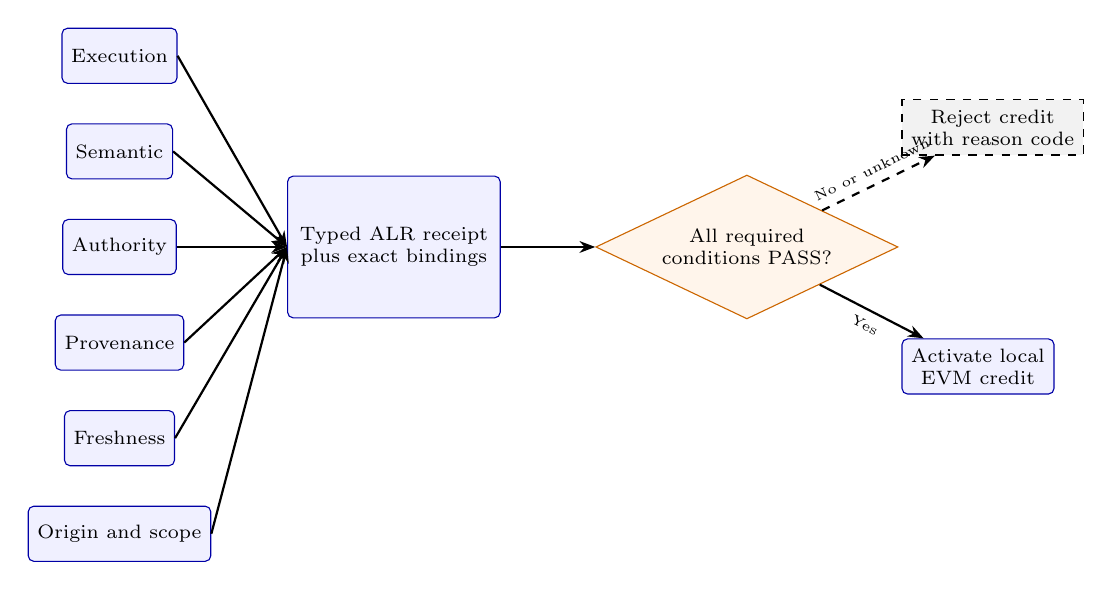
\begin{tikzpicture}[
  node distance=5mm and 6mm,
  box/.style={draw=blue!65!black, rounded corners=2pt, fill=blue!6, align=center, minimum height=7mm, font=\scriptsize},
  gate/.style={diamond, draw=orange!80!black, fill=orange!8, aspect=2.1, align=center, font=\scriptsize},
  reject/.style={draw=black, dashed, fill=gray!10, align=center, minimum height=7mm, font=\scriptsize},
  arrow/.style={-{Stealth[length=2mm]}, thick}
]
\node[box] (exec) {Execution};
\node[box, below=of exec] (sem) {Semantic};
\node[box, below=of sem] (auth) {Authority};
\node[box, below=of auth] (prov) {Provenance};
\node[box, below=of prov] (fresh) {Freshness};
\node[box, below=of fresh] (scope) {Origin and scope};
\node[box, right=14mm of auth, minimum width=27mm, minimum height=18mm] (receipt) {Typed ALR receipt\\plus exact bindings};
\node[gate, right=12mm of receipt] (meet) {All required\\conditions PASS?};
\node[reject, above right=7mm and 10mm of meet] (reject) {Reject credit\\with reason code};
\node[box, below right=7mm and 10mm of meet] (activate) {Activate local\\EVM credit};
\foreach \n in {exec,sem,auth,prov,fresh,scope} \draw[arrow] (\n.east) -- (receipt.west);
\draw[arrow] (receipt) -- (meet);
\draw[arrow,dashed] (meet) -- node[above,sloped,font=\tiny]{No or unknown} (reject);
\draw[arrow] (meet) -- node[below,sloped,font=\tiny]{Yes} (activate);
\end{tikzpicture}

}
\caption{ALR development architecture. Six typed assurance dimensions and seven
exact-binding predicates feed a non-compensating gate. Failure or unknown status
rejects credit with a deterministic reason; only all-pass input activates local EVM
credit. The diagram is architectural, not empirical evidence.}
\label{fig:architecture}
\end{figure}

\section{Methods}

\subsection{System and receipt rule}

The ALR contains six assurance dimensions: execution, semantic, authority,
provenance, freshness, and origin/scope. Each takes \texttt{PASS}, \texttt{FAIL}, or
\texttt{UNKNOWN}. Seven exact predicates cover unused-receipt status, request and
response hash bindings, authority-epoch liveness, allowed evidence origin,
claim-scope agreement, and type-tag validity. Eligibility is their conjunction
(Figure~\ref{fig:architecture}).

\subsection{Deterministic gate}

\begin{center}
\fbox{\begin{minipage}{0.92\linewidth}
\textbf{Algorithm 1: Fail-closed ALR eligibility.}
\begin{enumerate}[leftmargin=1.8em,itemsep=0.15em,topsep=0.25em]
\item For dimensions in the frozen order execution, semantic, authority,
provenance, freshness, and origin/scope: return its typed \texttt{FAIL} or
\texttt{UNKNOWN} reason at the first non-pass state.
\item Check, in order: receipt unused; request hash; response hash; live authority
epoch; allowed evidence origin; matching claim scope; valid type tag. Return the
corresponding rejection reason at the first failed predicate.
\item Return \texttt{ELIGIBLE} only if no rejection occurred.
\end{enumerate}
\end{minipage}}
\end{center}

The frozen order makes diagnostics deterministic. Consequently, reason-frequency
counts reflect precedence, not empirical risk or relative dimension importance.

\subsection{Design and analysis}

The base design is the complete Cartesian product $3^6=729$, a finite population
rather than a statistical sample. The all-pass tuple is the only eligible base state.
Seven additional fixtures introduce one exact-binding defect at a time. An oracle
transcription generates expected vectors separately from the Python reference kernel;
those vectors are compiled into the Solidity test. Missing or malformed rows count
as failures, and no rows are excluded or imputed. P-values and observed power are
inapplicable.

\begin{table}[t]
\centering
\caption{Development conditions and analysis populations.}
\label{tab:conditions}
\small
\begin{tabularx}{\linewidth}{@{}lYrr@{}}
\toprule
Condition & Definition & $n$ & Excluded \\
\midrule
Base & Complete six-dimension, three-level Cartesian product & 729 & 0 \\
Mutations & One failed binding with all six dimensions passing & 7 & Compound faults \\
Replay & Core artifacts compared across two same-owner processes & 3 & Timing logs \\
\bottomrule
\end{tabularx}
\end{table}

\subsection{Implementation and reproducibility}

The run used Python 3.14.6, Foundry 1.5.1-stable, and Solidity 0.8.24 on macOS 15.1
arm64. The runner captured argv, return codes, logs, and SHA-256 values without
network access. A second same-owner process replayed the workflow with a fixed
protocol timestamp (Figure~\ref{fig:workflow}). A subsequent producer-controlled
hermetic replay used a digest-pinned Linux amd64 image containing Foundry
1.5.1-v1.5.1 and exact Solidity 0.8.24. With network disabled, a read-only root and
case mount, dropped capabilities, and no new privileges, it reran the Python tests,
finite evaluation, generated-vector hash check, both Solidity parity tests, figures,
and manuscript build. This is reproducibility evidence, not independent replication.

\begin{figure}[t]
\centering
\resizebox{0.72\linewidth}{!}{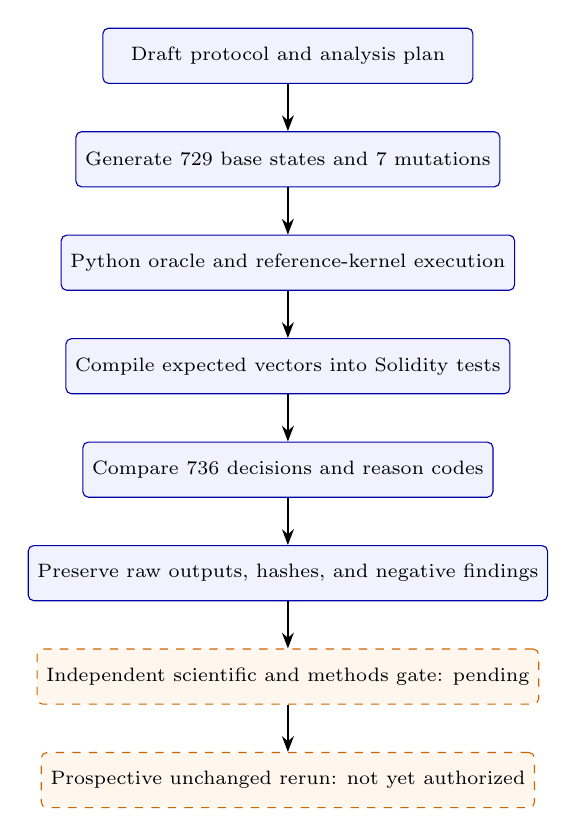
\begin{tikzpicture}[
  node distance=6mm,
  flowbox/.style={draw=blue!65!black, rounded corners=2pt, fill=blue!5, align=center, minimum width=47mm, minimum height=7mm, font=\scriptsize},
  pending/.style={draw=orange!80!black, dashed, rounded corners=2pt, fill=orange!7, align=center, minimum width=47mm, minimum height=7mm, font=\scriptsize},
  arrow/.style={-{Stealth[length=2mm]}, thick}
]
\node[flowbox] (protocol) {Draft protocol and analysis plan};
\node[flowbox, below=of protocol] (generate) {Generate 729 base states and 7 mutations};
\node[flowbox, below=of generate] (python) {Python oracle and reference-kernel execution};
\node[flowbox, below=of python] (solidity) {Compile expected vectors into Solidity tests};
\node[flowbox, below=of solidity] (compare) {Compare 736 decisions and reason codes};
\node[flowbox, below=of compare] (preserve) {Preserve raw outputs, hashes, and negative findings};
\node[pending, below=of preserve] (gate) {Independent scientific and methods gate: pending};
\node[pending, below=of gate] (rerun) {Prospective unchanged rerun: not yet authorized};
\foreach \a/\b in {protocol/generate,generate/python,python/solidity,solidity/compare,compare/preserve,preserve/gate,gate/rerun} \draw[arrow] (\a) -- (\b);
\end{tikzpicture}
}
\caption{Development workflow and open gate. The current evidence stops before
independent scientific/methods verification and a prospective unchanged rerun.}
\label{fig:workflow}
\end{figure}

\subsection{Ethics and evidence boundary}

The evaluation used synthetic state fixtures and locally authorized existing source
material. It involved no participants, personal data, live networks, or financial
transactions. Institutional and venue-specific determinations remain pending
accountable-human review.

\section{Results}

All 729 base states executed. The 728 ineligible states produced zero activations;
the all-pass state activated. Expected and observed base decisions and reasons agreed
for 729/729 states. All seven binding mutations rejected, and all 736 shared
Python-generated vectors matched Solidity outputs (Table~\ref{tab:results}). Three
Python unit tests and two Foundry tests passed.

\begin{table}[t]
\centering
\caption{Prespecified development outcomes. Intervals show finite-population observed
values, not sampling confidence intervals.}
\label{tab:results}
\small
\begin{tabularx}{\linewidth}{@{}Yrrl@{}}
\toprule
Outcome & Numerator & Denominator & Development decision \\
\midrule
False activations among ineligible states & 0 & 728 & Pass \\
Activation of all-pass state & 1 & 1 & Pass \\
Base decision and reason agreement & 729 & 729 & Pass \\
Mutation rejection & 7 & 7 & Pass \\
Python-generated vector/Solidity agreement & 736 & 736 & Pass \\
\bottomrule
\end{tabularx}
\end{table}

The same-owner replay reproduced identical SHA-256 values for the base CSV, mutation
CSV, and Python summary. Timing-bearing logs and run manifests differed as expected.
The hermetic replay returned zero for all eight declared commands, reproduced the
frozen Python hashes, passed both offline Foundry tests, and produced a venue-neutral
PDF byte-identical to the earlier pinned TeX build. These checks remain producer-owned.
Figure~\ref{fig:reasons} reports the first-reason distribution; its
486/162/54/18/6/2/1 pattern follows the fixed precedence and is not an empirical risk
ranking.

\begin{figure}[t]
\centering
\resizebox{0.94\linewidth}{!}{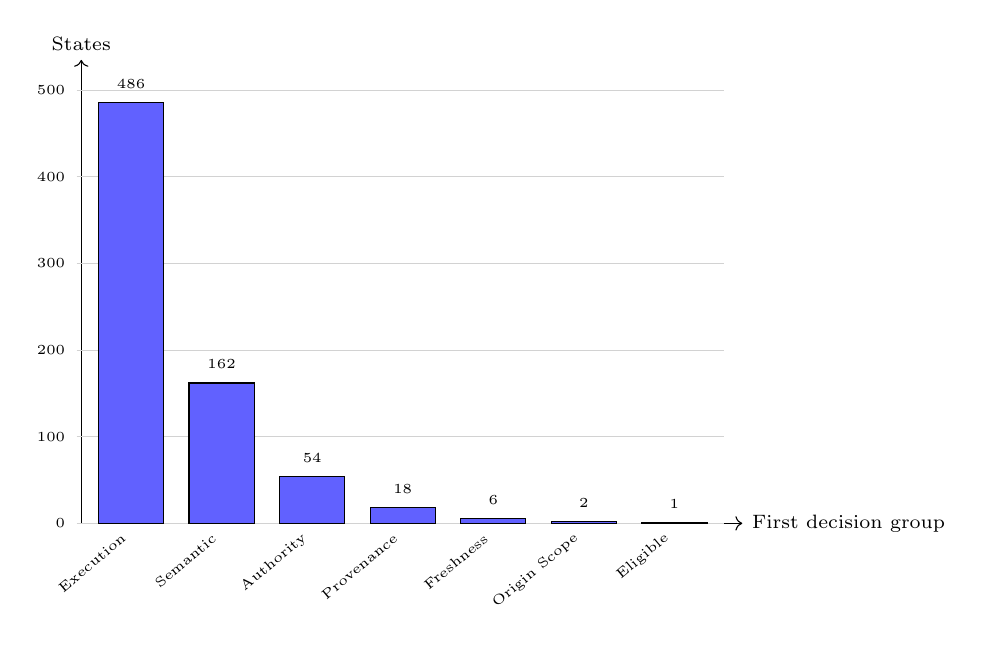
\begin{tikzpicture}[x=1.15cm,y=0.011cm]
\draw[->] (-0.55,0) -- (6.75,0) node[right,font=\scriptsize]{First decision group};
\draw[->] (-0.55,0) -- (-0.55,535) node[above,font=\scriptsize]{States};
\draw[gray!35] (-0.6,0) -- (6.55,0);
\node[anchor=east,font=\tiny] at (-0.62,0) {0};
\draw[gray!35] (-0.6,100) -- (6.55,100);
\node[anchor=east,font=\tiny] at (-0.62,100) {100};
\draw[gray!35] (-0.6,200) -- (6.55,200);
\node[anchor=east,font=\tiny] at (-0.62,200) {200};
\draw[gray!35] (-0.6,300) -- (6.55,300);
\node[anchor=east,font=\tiny] at (-0.62,300) {300};
\draw[gray!35] (-0.6,400) -- (6.55,400);
\node[anchor=east,font=\tiny] at (-0.62,400) {400};
\draw[gray!35] (-0.6,500) -- (6.55,500);
\node[anchor=east,font=\tiny] at (-0.62,500) {500};
\filldraw[fill=blue!62,draw=black] (-0.36,0) rectangle (0.36,486);
\node[font=\tiny,anchor=south] at (0,491) {486};
\node[font=\tiny,rotate=40,anchor=east] at (0,-8) {Execution};
\filldraw[fill=blue!62,draw=black] (0.64,0) rectangle (1.36,162);
\node[font=\tiny,anchor=south] at (1,167) {162};
\node[font=\tiny,rotate=40,anchor=east] at (1,-8) {Semantic};
\filldraw[fill=blue!62,draw=black] (1.64,0) rectangle (2.36,54);
\node[font=\tiny,anchor=south] at (2,59) {54};
\node[font=\tiny,rotate=40,anchor=east] at (2,-8) {Authority};
\filldraw[fill=blue!62,draw=black] (2.64,0) rectangle (3.36,18);
\node[font=\tiny,anchor=south] at (3,23) {18};
\node[font=\tiny,rotate=40,anchor=east] at (3,-8) {Provenance};
\filldraw[fill=blue!62,draw=black] (3.64,0) rectangle (4.36,6);
\node[font=\tiny,anchor=south] at (4,11) {6};
\node[font=\tiny,rotate=40,anchor=east] at (4,-8) {Freshness};
\filldraw[fill=blue!62,draw=black] (4.64,0) rectangle (5.36,2);
\node[font=\tiny,anchor=south] at (5,7) {2};
\node[font=\tiny,rotate=40,anchor=east] at (5,-8) {Origin Scope};
\filldraw[fill=orange!75,draw=black] (5.64,0) rectangle (6.36,1);
\node[font=\tiny,anchor=south] at (6,6) {1};
\node[font=\tiny,rotate=40,anchor=east] at (6,-8) {Eligible};
\end{tikzpicture}
}
\caption{First-decision reason groups across the complete 729-state base matrix.
Counts are deterministic products of Cartesian enumeration and the frozen precedence
rule. They do not measure prevalence, severity, or assurance importance. Underlying
data are in \texttt{reason-distribution-data.csv}.}
\label{fig:reasons}
\end{figure}

Several decisive outcomes remain negative or unresolved: independent protocol review
did not precede execution; no numeric gas comparator was frozen; malformed-type parity
is partial; independent reproduction and field validation were not performed; novelty
is unresolved; and the prior PoI semantic result remains \texttt{NOT\_SUPPORTED}
with FAR 0.500 against a frozen 0.25 threshold. The prior negative is retained as
context and not used as positive ALR evidence.

\clearpage
\section{Discussion}

Within the frozen model and seven named mutations, the Python and Solidity
implementations obeyed the prespecified fail-closed rule. This narrow conformance
result does not establish that the model captures every assurance dimension or
attack, that semantic input is correct, or that local behavior transports to
production. Assurance-case research likewise cautions that successful test processes
do not automatically warrant inferences from tested to fielded behavior
\cite{richard2026agentic}.

Novelty is especially uncertain. LATTICE overlaps deterministic governance gates and
auditable evidence chains; tool receipts overlap typed evidence sources; freshness
work overlaps replay-resistant evidence currency; and opML/EigenAI overlap blockchain
inference verification and enforcement. The remaining candidate difference is the
specific typed, non-compensating EVM receipt-to-credit composition and its exhaustive
development contract. Whether this is material or obvious requires independent
scientific judgment.

A prospective unchanged rerun after independent protocol review is the cheapest next
falsification step. A fair baseline must be frozen before any bounded-gas claim.
External reproduction can then test whether the artifact and instructions suffice
outside the producer's environment.

\section{Conclusion}

The ALR prototype provides exact development evidence for one deliberately narrow
claim: within the frozen finite model and seven named binding mutations, separately
implemented Python and Solidity decision paths conformed to the same fail-closed rule.
That result is useful as a falsifiable software contract, but it is not evidence of
semantic correctness, universal attack coverage, production safety, external
generality, or material novelty. The minimum responsible publication path is therefore
to preserve this claim ceiling while completing independent novelty and protocol
review, a prospective unchanged rerun, and external reproduction.

\section{Limitations}

The protocol and analysis plan were reviewed only within the producing AI-assisted
workflow. The finite model and mutation set may be incomplete. Neither the
fresh-directory nor hermetic producer replay is independent replication. The derived
container image is content-addressed locally but not publicly distributed. Foundry
test-call gas is not transaction or
production gas. The study did not evaluate semantic accuracy, decentralized
adversaries, mainnet conditions, privacy, TEEs, consensus safety, user outcomes, or
field impact. The bounded literature search awaits independent challenge,
patent/standard refresh, and full-text predecessor reconciliation. Authorship,
declarations, venue rules, and approval remain open.

\section{Data and code availability}

Development code, generated state tables, logs, manifests, figure data, Mermaid
source, and manuscript source are preserved locally in the research-system folder.
No public repository, archival DOI, license, or immutable release has been approved;
public availability is therefore pending human decision, not promised.

\section*{Declarations}

\textbf{Authorship and CRediT:} unresolved. Accountable humans must determine
eligibility, order, affiliations, and roles.\\
\textbf{Funding:} unverified.\\
\textbf{Competing interests:} unverified.\\
\textbf{Ethics:} software-only development evaluation with no human participants or
personal data; institutional applicability is not independently determined.\\
\textbf{AI use:} OpenAI Codex assisted with local code generation, execution,
analysis, visual-source preparation, and drafting. Accountable human authors must
verify all content and adapt disclosure to current venue policy.\\
\textbf{Submission approval:} not granted.

\bibliographystyle{plain}
\bibliography{references}

\end{document}
